\documentclass[tikz,border=4pt]{standalone}
\usepackage{tikz}
\usetikzlibrary{arrows.meta, positioning, shapes.geometric, backgrounds, fit, calc, decorations.pathreplacing}

\begin{document}
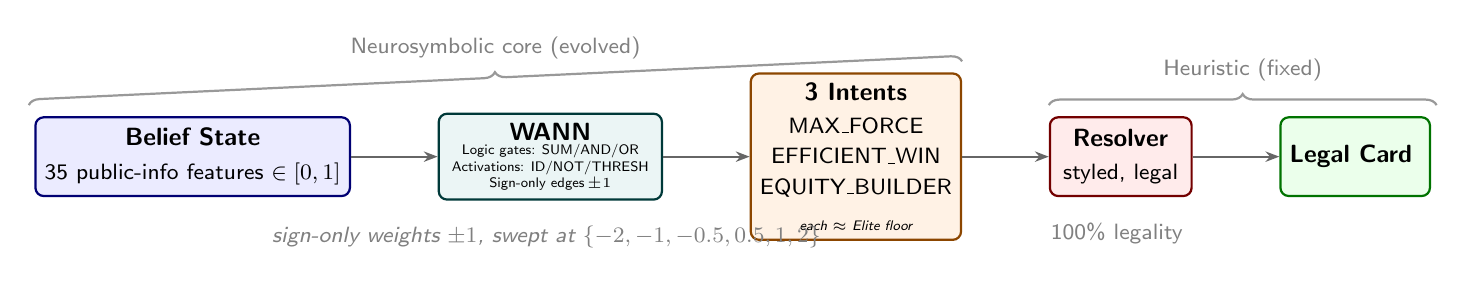
\begin{tikzpicture}[
    node distance=6mm and 11mm,
    box/.style={
      draw, thick, rounded corners=3pt,
      minimum width=22mm, minimum height=10mm,
      align=center, font=\small\sffamily
    },
    widebox/.style={
      box, minimum width=28mm
    },
    narrowbox/.style={
      box, minimum width=18mm
    },
    arrow/.style={
      -{Stealth[length=5pt]}, thick, black!60
    },
    label/.style={
      font=\footnotesize\sffamily\itshape, black!50
    },
    % Color palette — restrained, distinguishable hues
    % Stage 1: belief (blue-gray)
    % Stage 2: WANN (teal)
    % Stage 3: intents (amber)
    % Stage 4: resolver (burgundy)
    % Stage 5: card (green-gray)
    belief/.style={fill=blue!8, draw=blue!45!black},
    wann/.style={fill=teal!8, draw=teal!45!black},
    intent/.style={fill=orange!10, draw=orange!55!black},
    resolver/.style={fill=red!8, draw=red!45!black},
    card/.style={fill=green!8, draw=green!45!black},
    innerbox/.style={draw=black!25, rounded corners=1.5pt, fill=white, font=\tiny\sffamily, align=center, inner sep=2pt},
]

% === Stage 1: Belief State ===
\node[widebox, belief] (belief) {
  \textbf{Belief State}\\[1pt]
  \footnotesize 35 public-info features $\in [0,1]$
};

% === Stage 2: WANN ===
\node[widebox, wann, right=of belief] (wann) {
  \textbf{WANN}\\[1pt]
  \begin{minipage}{26mm}\centering\tiny
  Logic gates: SUM/AND/OR\\
  Activations: ID/NOT/THRESH\\
  Sign-only edges\,$\pm{}1$
  \end{minipage}
};

% === Stage 3: Intents ===
\node[narrowbox, intent, right=of wann] (intents) {
  \textbf{3 Intents}\\[1pt]
  \footnotesize MAX\_FORCE\\
  \footnotesize EFFICIENT\_WIN\\
  \footnotesize EQUITY\_BUILDER\\[2pt]
  {\tiny\itshape each $\approx$ Elite floor}
};

% === Stage 4: Resolver ===
\node[narrowbox, resolver, right=of intents] (resolver) {
  \textbf{Resolver}\\[1pt]
  \footnotesize styled, legal
};

% === Stage 5: Card ===
\node[narrowbox, card, right=of resolver] (card) {
  \textbf{Legal Card}
};

% === Arrows between stages ===
\draw[arrow] (belief) -- (wann);
\draw[arrow] (wann) -- (intents);
\draw[arrow] (intents) -- (resolver);
\draw[arrow] (resolver) -- (card);

% === Annotation: WANN internals ===
\node[label, below=2mm of wann.south, align=center] {
  \footnotesize sign-only weights $\pm{}1$, swept at $\{-2,-1,-0.5,0.5,1,2\}$
};

% === Annotation: resolver guarantee ===
\node[label, below=2mm of resolver.south, align=center, font=\footnotesize\sffamily] {
  100\% legality
};

% === Braces for phases ===
\draw [decorate, decoration={brace, amplitude=4pt}, black!40, thick]
  ($(belief.north west) + (-2pt, 4pt)$) -- ($(intents.north east) + (0pt, 4pt)$)
  node[midway, above=5pt, font=\footnotesize\sffamily, black!50] {Neurosymbolic core (evolved)};

\draw [decorate, decoration={brace, amplitude=4pt}, black!40, thick]
  ($(resolver.north west) + (0pt, 4pt)$) -- ($(card.north east) + (2pt, 4pt)$)
  node[midway, above=5pt, font=\footnotesize\sffamily, black!50] {Heuristic (fixed)};

\end{tikzpicture}
\end{document}
